\documentclass[a4paper,12pt]{article}

% Packages essentiels
\usepackage{lmodern} % police vectorielle
\usepackage[protrusion=true, expansion=true]{microtype}
\usepackage[french]{babel}
\usepackage[T1]{fontenc} 
\usepackage[utf8]{inputenc}
\usepackage{csquotes} % recommandé avec biblatex 
\usepackage{algorithm}
\usepackage{algorithmic}

% Math et symboles
\usepackage{amsmath}
\usepackage{amssymb} 

% Figures et tableaux
\usepackage{graphicx}
\usepackage{subcaption}
\usepackage{multirow}
\usepackage{float} 

% Mise en page
\usepackage{geometry} 
\usepackage{titlesec}
\setcounter{secnumdepth}{4}
\titleformat{\paragraph}
{\normalfont\normalsize\bfseries}{\theparagraph}{1em}{}
\titlespacing*{\paragraph}
{0pt}{3.25ex plus 1ex minus .2ex}{1.5ex plus .2ex}

\geometry{top=2cm, bottom=2cm, left=2cm, right=2cm}

\usepackage[table,dvipsnames]{xcolor}
\usepackage{hyperref} 
\hypersetup{colorlinks=true, linkcolor=black, citecolor=gray, urlcolor=blue}

\usepackage{siunitx}
\sisetup{output-decimal-marker = {,}, group-separator = {\,}, group-minimum-digits = 4}

\usepackage[style=apa, backend=biber, sorting=nyt, natbib=false]{biblatex}
\addbibresource{references.bib}

\usepackage{tocloft}
\setlength{\cftbeforesecskip}{10pt}
\setlength{\cftbeforesubsecskip}{8pt}
\renewcommand{\cftsecleader}{\cftdotfill{\cftdotsep}}
\setlength{\cftaftertoctitleskip}{25pt}

\title{ADAM pour le Deep Learning}
\author{ACHIQ Aya, CLETZ Laura, EL MAZZOUJI Wahel}
\date{Octobre 2025}

\begin{document}

\begin{titlepage}
\centering

\begin{minipage}{0.4\textwidth}
    
\includegraphics[width=\linewidth]{images/FdS.jpg}
\end{minipage}
\hfill
\begin{minipage}{0.4\textwidth}
    
\includegraphics[width=\linewidth]{images/UM.png}
\end{minipage}

\vspace{1cm}

\begin{minipage}{0.4\textwidth}
    \centering
    
\includegraphics[width=\linewidth]{images/SSD.png}
\end{minipage}

\vspace{2cm}

{\Large Lecture d'article}\\[0.4cm]
{\LARGE \textbf{ADAM pour le Deep Learning}}\\[1.2cm]

{\large Groupe :}\\[0.3cm]
\textbf{ACHIQ Aya}\\
\textbf{CLETZ Laura}\\
\textbf{EL MAZZOUJI Wahel}\\[1.5cm]

{\large Octobre 2025}

\vfill
\end{titlepage}

\newpage
\tableofcontents
\listoffigures
\listoftables
\newpage

\section{Introduction}

L’optimisation occupe une place essentielle dans l’apprentissage
profond, où la descente de gradient stochastique et ses variantes à
momentum ont longtemps été les méthodes de référence. Cependant, ces
approches présentent certaines limites, car leur convergence peut être
lente et leur performance dépend fortement du choix du taux
d’apprentissage, souvent difficile à ajuster.

Pour pallier ces difficultés, des méthodes dites adaptatives ont été
proposées, comme AdaGrad et RMSProp, qui ajustent automatiquement le pas
d’apprentissage pour chaque paramètre. Parmi elles, l’algorithme Adam
\cite{kingma2014} s’est imposé comme un compromis efficace entre
rapidité et stabilité, devenant l’une des méthodes les plus utilisées en
apprentissage profond.

Néanmoins, plusieurs travaux récents, notamment ceux de \cite{wilson2017}, ont remis en question la supériorité généralisée de ces
approches adaptatives. Ce rapport s’interroge sur la validité de cette
hypothèse et cherche à déterminer si les méthodes adaptatives telles
qu’Adam sont réellement plus performantes que les méthodes non
adaptatives comme SGD, tant en termes de convergence que de
généralisation.


\section{Adam et les méthodes adaptatives}

\subsection{Contexte et motivation}

L'apprentissage profond repose sur la minimisation stochastique d'une fonction de coût
bruitée. La descente de gradient stochastique et ses variantes à momentum sont simples
mais sensibles au choix du taux d'apprentissage et instables en présence de gradients bruités
ou clairsemés. Pour pallier ces limites, Adam (\emph{Adaptive Moment Estimation}) a été
proposé par \cite{kingma2014}. L'idée est de combiner les avantages du momentum (cf annexes \ref{annexes}) et de
l'adaptation du taux d'apprentissage, comme dans AdaGrad et RMSProp (cf annexes \ref{annexes}), afin d'obtenir une
descente plus rapide et plus stable.

Cependant, plusieurs travaux ont montré que la rapidité de convergence des méthodes
adaptatives ne garantit pas toujours une meilleure généralisation. \cite{wilson2017}
soulignent que ces méthodes peuvent conduire à des minima différents de ceux trouvés par
SGD, parfois moins performants sur les données de test.

\subsection{Principe de l’algorithme Adam}

L’algorithme Adam combine deux idées
majeures : l’accumulation du momentum et l’adaptation du taux
d’apprentissage pour chaque paramètre. À chaque itération $t$, le gradient stochastique
$g_t = \nabla_\theta f_t(\theta_{t-1})$ sert à mettre à jour deux
moyennes mobiles :
$m_t = \beta_1 m_{t-1} + (1-\beta_1) g_t$ et
$v_t = \beta_2 v_{t-1} + (1-\beta_2) g_t^2$,
où $m_t$ représente la moyenne et $v_t$ la variance du gradient. Les coefficients usuels sont
$\beta_1=0.9$ et $\beta_2=0.999$. Comme $m_0$ et $v_0$ sont initialisés
à zéro, \cite{kingma2014} introduisent une correction de biais :
$\hat{m}_t = m_t/(1-\beta_1^t)$ et
$\hat{v}_t = v_t/(1-\beta_2^t)$.

La mise à jour s’écrit
\[
\theta_t = \theta_{t-1} - \alpha\,\frac{\hat{m}_t}{\sqrt{\hat{v}_t}+\varepsilon},
\]
où $\alpha$ est le taux d’apprentissage et $\varepsilon\approx10^{-8}$ évite la division par zéro.
Cette règle combine la direction moyenne du gradient (momentum) et une
normalisation par la variance locale, assurant une descente rapide et
stable face aux variations d’échelle.
L’algorithme complet est présenté en Annexe pour référence.


\subsection{Interprétation et propriétés}

Adam combine momentum et adaptation du pas : $m_t$ lisse la direction de
descente, tandis que $v_t$ ajuste le pas selon la variance locale du
gradient, réduisant les oscillations et stabilisant l’entraînement.

Adam présente plusieurs propriétés remarquables. Il est invariant à
l’échelle des gradients, son pas est borné et contrôlé par $\alpha$, et
il reste peu sensible aux hyperparamètres. \cite{kingma2014} montrent, dans
le cadre convexe, un regret en $\mathcal{O}(\sqrt{T})$, équivalent à
AdaGrad mais plus stable sur des objectifs non stationnaires.

Ces propriétés expliquent la popularité d’Adam pour l’apprentissage de
réseaux profonds, où les gradients peuvent être bruités, corrélés ou
fortement déséquilibrés selon les paramètres.

\subsection{Forces et apports de la méthode Adam}

Les expériences de \cite{kingma2014} sur diverses tâches, telles que
la régression logistique et l’apprentissage de réseaux profonds,
montrent qu’Adam combine la rapidité d’AdaGrad et la stabilité
de RMSProp. Sur MNIST, il atteint une faible perte en peu d’itérations
et une précision comparable à SGD avec momentum, sans réglage manuel du
taux d’apprentissage.

L’algorithme se distingue par sa robustesse aux hyperparamètres, sa rapidité de convergence et son efficacité face à des gradients bruités. Les valeurs par défaut
($\alpha\!=\!0.001$, $\beta_1\!=\!0.9$, $\beta_2\!=\!0.999$,
$\varepsilon\!=\!10^{-8}$) offrent de bonnes performances dans la
plupart des contextes, ce qui explique sa popularité comme méthode
d’optimisation de référence en apprentissage profond.

Enfin, la variante AdaMax, fondée sur la norme infinie, améliore la stabilité numérique tout en conservant la simplicité d’Adam.

\subsection{Limites théoriques}

Bien qu’efficace en pratique, Adam présente une généralisation
limitée. \cite{wilson2017} montrent que les méthodes adaptatives
diffèrent des approches non adaptatives comme SGD.

Théoriquement, \cite{wilson2017} montrent que SGD converge vers une
\emph{solution à norme minimale} ($\|w\|_2$ faible), gage d’une bonne
généralisation, tandis que les méthodes adaptatives tendent vers des
\emph{solutions à norme infinie minimale} ($\|w\|_\infty$ faible),
souvent associées à un surapprentissage.

\cite{wilson2017} montrent qu’Adam peut converger vers des solutions
mal généralisées, alors que SGD atteint la solution optimale, ce qui
explique la moindre généralisation des méthodes adaptatives.

Ces travaux soulignent ainsi le compromis fondamental entre rapidité d’apprentissage et capacité de généralisation propre aux méthodes adaptatives.

\section{Expériences et comparaisons}

Suivant les résultats théoriques comparatifs de \cite{wilson2017}, nous allons comparer sur deux bases de données connues les méthodes Adam et SGD, mais aussi deux méthodes proches : Adagrad et RMSprop. L'ensemble des tableaux et des graphes sont disponibles en annexes \ref{annexes}.
\par Nous entraînerons les modèles avec les quatre optimiseurs en utilisant les taux d'apprentissage standards recommandés dans la littérature (\cite{ruder2016overview}) : Adam ($\eta$=0.001), SGD ($\eta$=0.01), Adagrad ($\eta$=0.01) et RMSprop ($\eta$=0.001).

\subsection{Base de données "Credit Card Fraud Detection"}

Pour comparer les performances des quatre méthodes citées, nous commençons avec la base de données "Credit Card Fraud Detection". C'est une base de données publique disponible sur Kaggle\footnote{\url{https://www.kaggle.com/datasets/mlg-ulb/creditcardfraud}} qui contient des transactions par carte de crédit, dont certaines sont frauduleuses. Le but est de détecter ces fraudes à partir des caractéristiques des transactions. 
\par Nous gardons les variables "V14" et "Amount" comme variables explicatives, elles représentent respectivement les résultats d'une ACP (Analyse en Composantes Principales) anonymisant ainsi les données d'utilisation et d'utilisateur.ice de la carte qui sont fortement corrélés à la fraude, et le montant de la transaction. La variable "Class" est la variable réponse où $0$ signifie que la transaction est légitime et $1$ est une fraude. 
\par Nous utilisons un réseau de neurones simple avec une couche cachée de 16 neurones et une fonction d'activation ReLU (cf cours GLM). La fonction de perte "\texttt{binary cross-entropy}" est en fait celle associée à la régression logistique (cf annexes \ref{annexes}).\\

Les tableaux~\ref{tab:results_10k} et~\ref{tab:results_100k} révèlent plusieurs tendances intéressantes : 
\par Sur un $10\,000$-échantillon, chaque méthode sur-ajuste sur l'entraînement donc les résultats pour les précisions sur l'ensemble de test sont égaux. Adam obtient cependant la meilleure perte de test (0.0057), avec un facteur 10 plus petit par rapport aux autres méthodes. 
\par Sur un $100\,000$-échantillon, Adam domine de peu avec une précision remarquable de 99.91\% et une perte de test de 0.0033. Adagrad et RMSprop montrent de meilleurs performances sur ce plus grand échantillon.
\par Il semble ainsi que l'augmentation de la taille d'échantillon favorise nettement les performances de chaque modèle, confirmant leur robustesse sur des datasets plus importants, pourtant nous n'apercevons pas d'amélioration évidente pour Adam.
\par Graphiquement, ces observations se confirment à travers l'évolution des métriques d'entraînement et de test. La figure~\ref{fig:training_comparison} illustre l'évolution de l'erreur d'entraînement (cf annexes \ref{annexes}) au cours des \textit{epochs}, révélant les vitesses de convergence distinctes de chaque optimiseur.
\par On observe qu'Adagrad converge rapidement vers une faible erreur initiale, mais stagne ensuite, tandis qu'Adam continue à améliorer l'erreur au fil des \textit{epochs}. Adagrad converge le plus lentement, RMSprop plus rapidement, et à partir de 2 epochs, SGD ne présente pas de claire convergence.
La figure~\ref{fig:test_results} présente une synthèse des performances finales de test, mettant en évidence les différences de généralisation entre les méthodes selon la taille de l'échantillon.
\par Ces visualisations confirment qu'Adam maintient des performances robustes à travers les différentes tailles d'échantillon, tandis qu'SGD, malgré une convergence similaire sur le grand échantillon, voit ses performances se dégrader légèrement avec l'augmentation des données.

\subsection{Base de données "Heart Disease"}
Pour valider les optimiseurs dans un contexte différent, nous utilisons le dataset Heart Disease, disponible sur Kaggle\footnote{\url{https://www.kaggle.com/datasets/fedesoriano/heart-failure-prediction}}. Ce dataset contient 1025 observations de patients avec 13 caractéristiques cliniques (âge, sexe, pression artérielle, cholestérol, etc.) permettant de prédire la présence de maladie cardiaque. La variable cible est binaire : 0 pour absence de maladie, 1 pour présence. Les classes sont relativement équilibrées (49\% / 51\%).

Nous utilisons un réseau de neurones avec deux couches cachées (16 et 8 neurones) et activation ReLU, suivi d'une couche de sortie avec activation sigmoid. La fonction de perte utilisée est la binary cross-entropy. L'entraînement se fait sur 100 epochs avec batch size de 32 et validation split de 20\%. Un mécanisme d'early stopping (patience=10) est implémenté pour prévenir le surapprentissage.

\par Le tableau \ref{tab:heart} présente les performances finales sur l'ensemble de test. Les résultats révèlent que RMSprop obtient la meilleure précision (94.16\%), suivi de près par Adam (93.18\%). SGD affiche des performances nettement inférieures (80.84\%), tandis qu'Adagrad se situe en position intermédiaire (88.64\%). \\

\par Graphiquement, ces observations se confirment à travers l'évolution des métriques d'entraînement et de test. La figure \ref{fig:heart_err} illustre l'évolution de l'erreur au cours des epochs, révélant les vitesses de convergence distinctes de chaque optimiseur. On observe que RMSprop et Adam convergent rapidement et régulièrement vers de faibles erreurs, tandis que SGD montre une convergence plus lente et moins stable. Adagrad converge initialement de manière rapide mais stagne ensuite. \\

\par La figure \ref{fig:heart_loss} présente l'évolution de la perte, confirmant ces observations.

\par Ces résultats contrastent fortement avec ceux obtenus sur Credit Card où Adam, Adagrad et RMSprop affichaient des performances quasi-identiques (99.91\%). Cette différence s'explique par plusieurs facteurs : la taille réduite du dataset (1025 vs 100 000 observations) où SGD souffre davantage du bruit stochastique, et la dimensionnalité accrue (13 vs 2 features) qui favorise l'adaptation locale du taux d'apprentissage. Les méthodes adaptatives (RMSprop, Adam) démontrent ainsi leur supériorité sur des datasets de taille modeste et de dimension élevée, confirmant leur robustesse aux hyperparamètres et leur efficacité face à des gradients hétérogènes.

\section{Conclusion}

Ce travail a étudié l’algorithme Adam à travers ses fondements
théoriques et ses performances pratiques. Proposé par
\cite{kingma2014}, Adam combine momentum et adaptation du taux
d’apprentissage, assurant une convergence rapide et stable, même en
présence de gradients bruités. Cependant, comme l’ont montré
\cite{wilson2017}, cette efficacité ne garantit pas toujours une
meilleure généralisation, les solutions obtenues pouvant différer de
celles issues de méthodes non adaptatives comme SGD. Nos expériences montrent d'ailleurs que les performances des méthodes non-adaptatives dépendent fortement des caractéristiques du jeu de données, comme sa taille ou sa complexité.


Les expériences confirment ce compromis entre rapidité et
généralisation, suggérant qu’Adam est bien adapté aux phases
d’entraînement initial, tandis que SGD demeure plus fiable pour la
généralisation. L’étude de variantes récentes, telles qu’AdamW ou
RAdam, pourrait permettre un meilleur équilibre entre ces deux aspects.




\newpage

\appendix
\section{Annexes}
\label{annexes}

\subsection{Graphiques}

\begin{figure}[H]
\centering
\begin{subfigure}[b]{0.48\textwidth}
    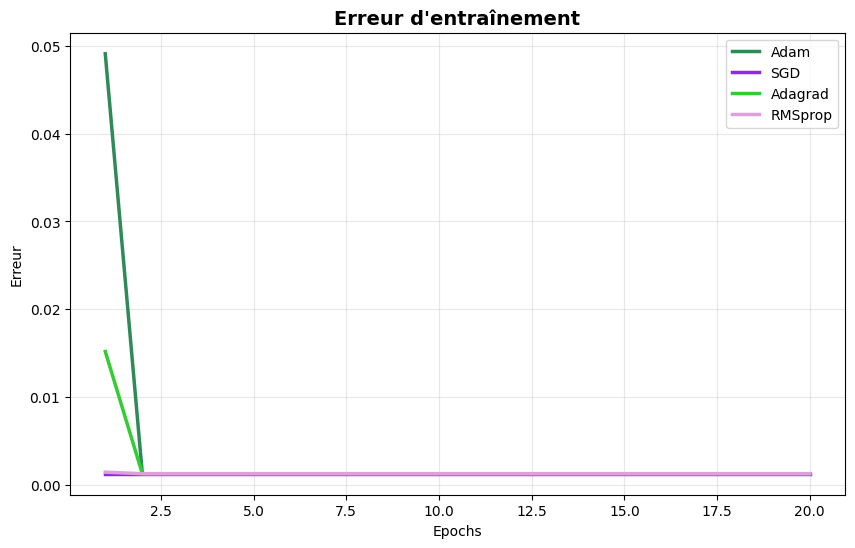
\includegraphics[width=\textwidth]{images/training_error_n10k.png}
    \caption[Erreur d'entraînement (n=10k)]{Erreur d'entraînement}
    \label{fig:training_10k}
\end{subfigure}
\hfill
\begin{subfigure}[b]{0.48\textwidth}
    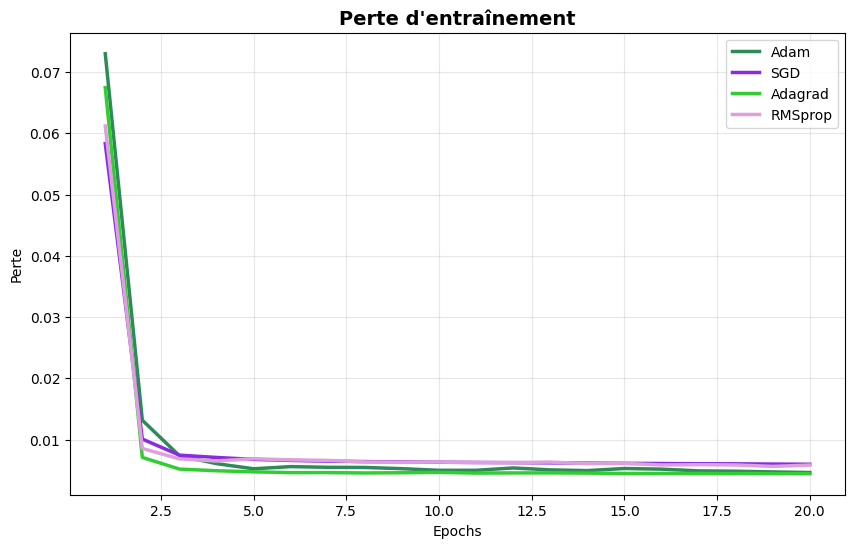
\includegraphics[width=\textwidth]{images/training_loss_n10k.png}
    \caption[Perte d'entraînement (n=10k)]{Perte d'entraînement}
    \label{fig:loss_10k}
\end{subfigure}
\caption{Comparaison des métriques d'entraînement pour $n=10\,000$}
\label{fig:training_comparison}
\end{figure}

\begin{figure}[H]
\centering
\begin{subfigure}[b]{0.48\textwidth}
    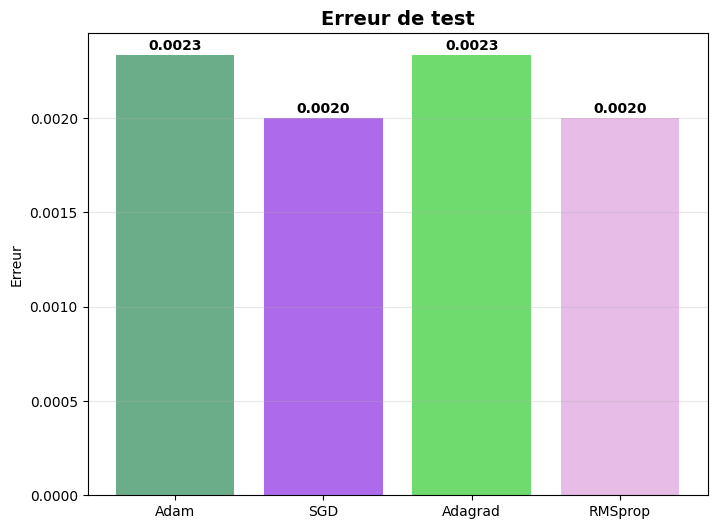
\includegraphics[width=\textwidth]{images/test_error_n10k.png}
    \caption[Erreurs de test (n=10k)]{Erreurs de test ($n=10\,000$)}
    \label{fig:test_10k}
\end{subfigure}
\hfill
\begin{subfigure}[b]{0.48\textwidth}
    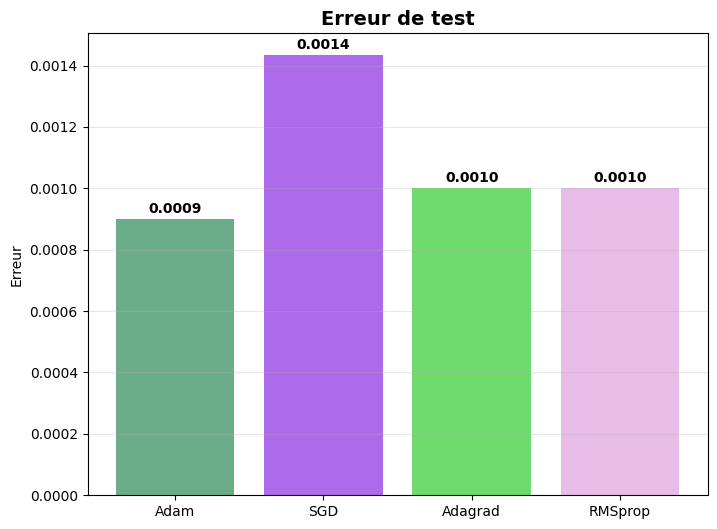
\includegraphics[width=\textwidth]{images/test_error_n100k.png}
    \caption[Erreurs de test (n=100k)]{Erreurs de test ($n=100\,000$)}
    \label{fig:test_100k}
\end{subfigure}
\caption{Comparaison des erreurs de test finales}
\label{fig:test_results}
\end{figure}

\begin{figure}[H]
\centering
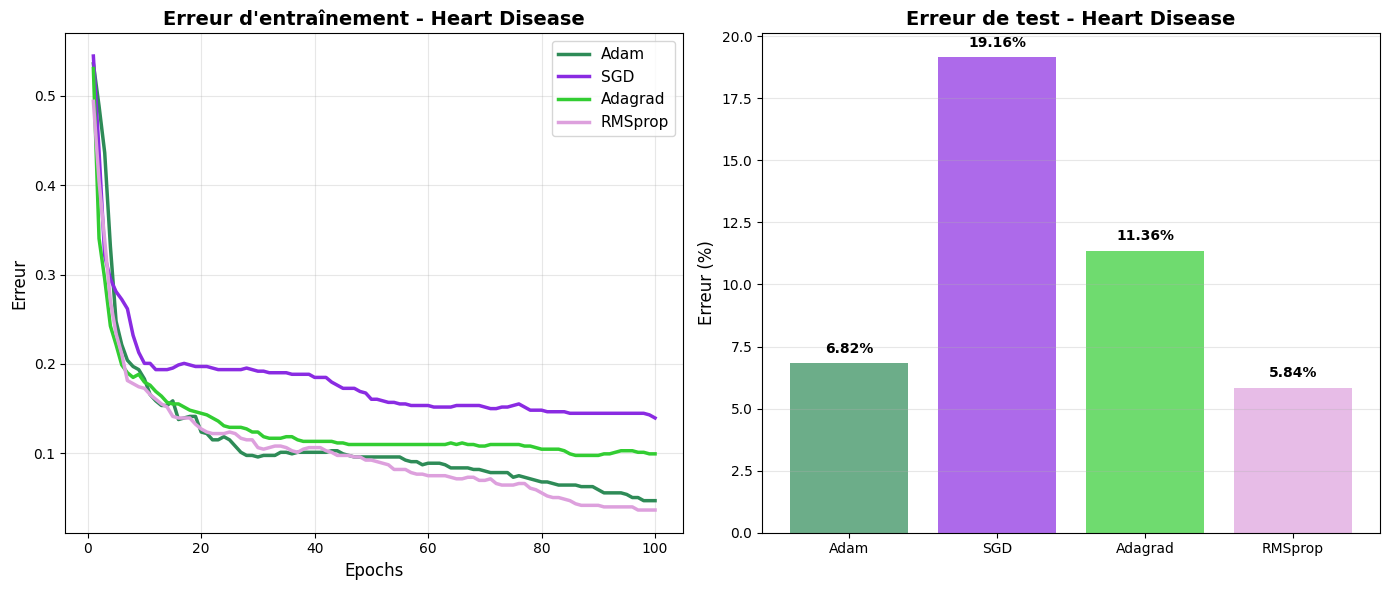
\includegraphics[width=\textwidth]{images/heart_errors.png}
\caption{Comparaison des erreurs pour Heart Disease}
\label{fig:heart_err}
\end{figure}

\begin{figure}[H]
\centering
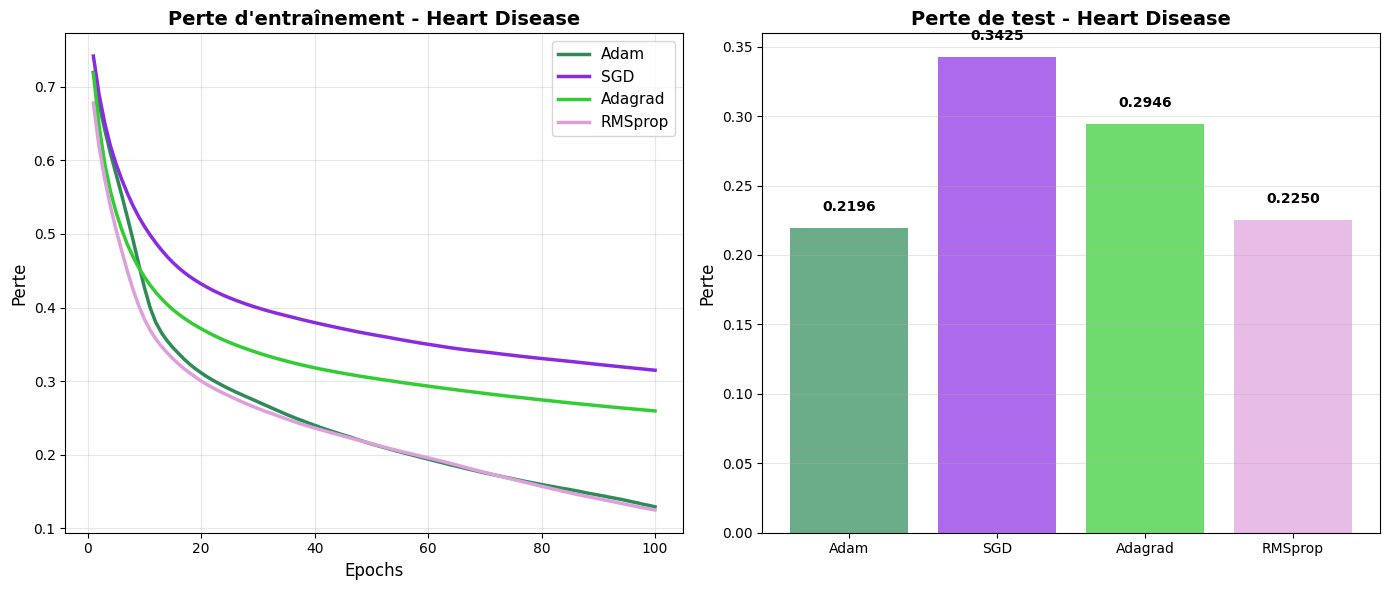
\includegraphics[width=\textwidth]{images/heart_losses.png}
\caption{Comparaison des pertes pour Heart Disease}
\label{fig:heart_loss}
\end{figure}

\subsection{Tableaux}

\begin{table}[H]
\centering
\begin{tabular}{|l|c|c|c|}
\hline
\rowcolor{lightgray}
\textbf{Optimiseur} & \textbf{Test Loss} & \textbf{Test Accuracy} & \textbf{Erreur de test (\%)} \\
\hline
\rowcolor{lightgray!50}
Adam      & 0.0057 & 0.9977 & 0.23 \\
\hline
SGD       & 0.0224 & 0.9977 & 0.23 \\
\hline
Adagrad   & 0.0271 & 0.9977 & 0.23 \\
\hline
RMSprop   & 0.0167 & 0.9977 & 0.23 \\
\hline
\end{tabular}
\caption{Comparaison des performances sur l'échantillon de taille $n=10\,000$}
\label{tab:results_10k}
\end{table}

\begin{table}[H]
\centering
\begin{tabular}{|l|c|c|c|}
\hline
\rowcolor{lightgray}
\textbf{Optimiseur} & \textbf{Test Loss} & \textbf{Test Accuracy} & \textbf{Erreur de test (\%)} \\
\hline
\rowcolor{lightgray!50}
Adam      & 0.0033 & \textbf{0.9991} & \textbf{0.09} \\
\hline
SGD       & 0.0046 & 0.9986 & 0.14 \\
\hline
Adagrad   & 0.0042 & 0.9990 & 0.1 \\
\hline
RMSprop   & 0.0045 & 0.9990 & 0.1 \\
\hline
\end{tabular}
\caption{Comparaison des performances sur l'échantillon de taille $n=100\,000$}
\label{tab:results_100k}
\end{table}

\begin{table}[H]
\centering
\begin{tabular}{|l|c|c|c|}
\hline
\rowcolor{lightgray}
\textbf{Optimiseur} & \textbf{Test Loss} & \textbf{Test Accuracy} & \textbf{Erreur (\%)} \\
\hline
Adam      & 0.2196 & 0.9318 & 6.82 \\
\hline
SGD       & 0.3425 & 0.8084 & 19.16 \\
\hline
Adagrad   & 0.2946 & 0.8864 & 11.36 \\
\hline
\rowcolor{lightgray!50}
RMSprop   & \textbf{0.2250} & \textbf{0.9416} & \textbf{5.84} \\
\hline
\end{tabular}
\caption{Comparaison des performances sur Heart Disease ($n=1\,025$)}
\label{tab:heart}
\end{table}

\subsection{Définitions et formules}

\noindent\textbf{Gradient non adaptatif}\\
\par Une méthode non adaptative utilise un taux d'apprentissage fixe $\eta$ identique pour tous les paramètres
et à toutes les itérations :
\[
\theta_{t+1} = \theta_t - \eta \, g_t,
\]
où $g_t = \nabla_\theta f_t(\theta_t)$ est le gradient de la fonction de coût.\\

\noindent\textbf{Gradient adaptatif}\\
\par Une méthode adaptative ajuste dynamiquement le taux d’apprentissage
pour chaque paramètre en fonction de l’historique de ses gradients.
Les paramètres dont les gradients varient fortement reçoivent un pas plus
petit, ceux dont les gradients sont faibles un pas plus grand :
\[
\theta_{t+1} = \theta_t - \frac{\eta}{\sqrt{v_t} + \epsilon} \, g_t,
\]
avec $v_t$ la moyenne des carrés des gradients passés.\\

\noindent\textbf{Momentum}\\
\par Le momentum ajoute une mémoire du gradient passé pour lisser la
trajectoire de la descente :
\[
m_t = \beta_1 m_{t-1} + (1 - \beta_1) g_t.
\]
Ce mécanisme stabilise la descente et permet d’atteindre plus facilement le minimum.\\

\noindent\textbf{Adagrad}\\
\par Adagrad adapte le taux d’apprentissage en fonction de l’historique des
gradients :
\[v_t = v_{t-1} + g_t^2,
\]
où $v_t$ est la somme des carrés des gradients. La mise à jour devient
\[\theta_{t+1} = \theta_t - \frac{\eta}{\sqrt{v_t} + \epsilon} \, g_t.
\] \\

\noindent\textbf{RMSprop}\\
\par RMSProp modifie Adagrad en utilisant une moyenne mobile exponentielle
des carrés des gradients :
\[v_t = \beta_2 v_{t-1} + (1 - \beta_2) g_t^2,
\]
avec $\beta_2$ proche de 1. La mise à jour est la même.\\

\noindent\textbf{Régression logistique}\\
\par La régression logistique est un type de régression dans les cas binaires. Sa fonction de perte est définie par 
$$
L(y, \hat{y}) = -[y \log(\hat{y}) + (1-y) \log(1-\hat{y})]
$$  
avec $y\in{0,1}$ et $\hat{y}=\sigma(z)$ la probabilité prédite via la fonction sigmoid $\sigma(z) = 1/(1 + e^{-z})$. \\

\noindent\textbf{Erreur d'entraînement et perte}\\
\par L'erreur d'entraînement est la proportion de prédictions incorrectes sur l'ensemble d'entraînement, soit $1-$ la précision durant l'entraînement (\textit{training accuracy}), tandis que la perte mesure la qualité globale des prédictions.\\


\subsection{Algorithme Adam}

\begin{algorithm}[h]
\caption{Algorithme \textsc{Adam} (\cite{kingma2014})}
\begin{algorithmic}[1]
\REQUIRE $\alpha$ : pas d'apprentissage
\REQUIRE $\beta_1, \beta_2 \in [0,1)$ : taux de décroissance exponentielle des moments
\REQUIRE $f(\theta)$ : fonction objectif stochastique à minimiser
\REQUIRE $\theta_0$ : vecteur initial des paramètres
\STATE Initialiser $m_0 \leftarrow 0$ (1\textsuperscript{er} moment)
\STATE Initialiser $v_0 \leftarrow 0$ (2\textsuperscript{e} moment)
\STATE Initialiser $t \leftarrow 0$ (pas de temps)
\WHILE{$\theta_t$ non convergé}
    \STATE $t \leftarrow t + 1$
    \STATE Calculer $g_t = \nabla_\theta f_t(\theta_{t-1})$ \hfill (gradient au pas $t$)
    \STATE $m_t = \beta_1 m_{t-1} + (1 - \beta_1) g_t$ \hfill (moyenne mobile du gradient)
    \STATE $v_t = \beta_2 v_{t-1} + (1 - \beta_2) g_t^2$ \hfill (moyenne mobile des carrés)
    \STATE $\hat{m}_t = \frac{m_t}{1 - \beta_1^t}$ \hfill (correction de biais du 1\textsuperscript{er} moment)
    \STATE $\hat{v}_t = \frac{v_t}{1 - \beta_2^t}$ \hfill (correction de biais du 2\textsuperscript{e} moment)
    \STATE $\theta_t = \theta_{t-1} - \alpha \frac{\hat{m}_t}{\sqrt{\hat{v}_t} + \varepsilon}$ \hfill (mise à jour des paramètres)
\ENDWHILE
\RETURN $\theta_t$ (paramètres optimisés)
\end{algorithmic}
\end{algorithm}

\noindent\textbf{Remarques.} Toutes les opérations sur les vecteurs sont effectuées élément par élément.
Les valeurs par défaut recommandées sont $\alpha = 0{.}001$,
$\beta_1 = 0{.}9$, $\beta_2 = 0{.}999$ et $\varepsilon = 10^{-8}$.

\printbibliography

\end{document}